% Is missing images 6-9
\section{Praktiska tillämpningar}
Inom klassisk mekanik studeras så kallade "stela kroppar", dvs. objekt som kan tänkas fullständigt oelastiska där inbördes relativa asvtånd är oförändrade under påverkan av yttre krafter.
För dessa r \underline{tyngdpunkt} ett centralt och viktigt begrepp.
För partikelsystem:\\
% infoga bild 1
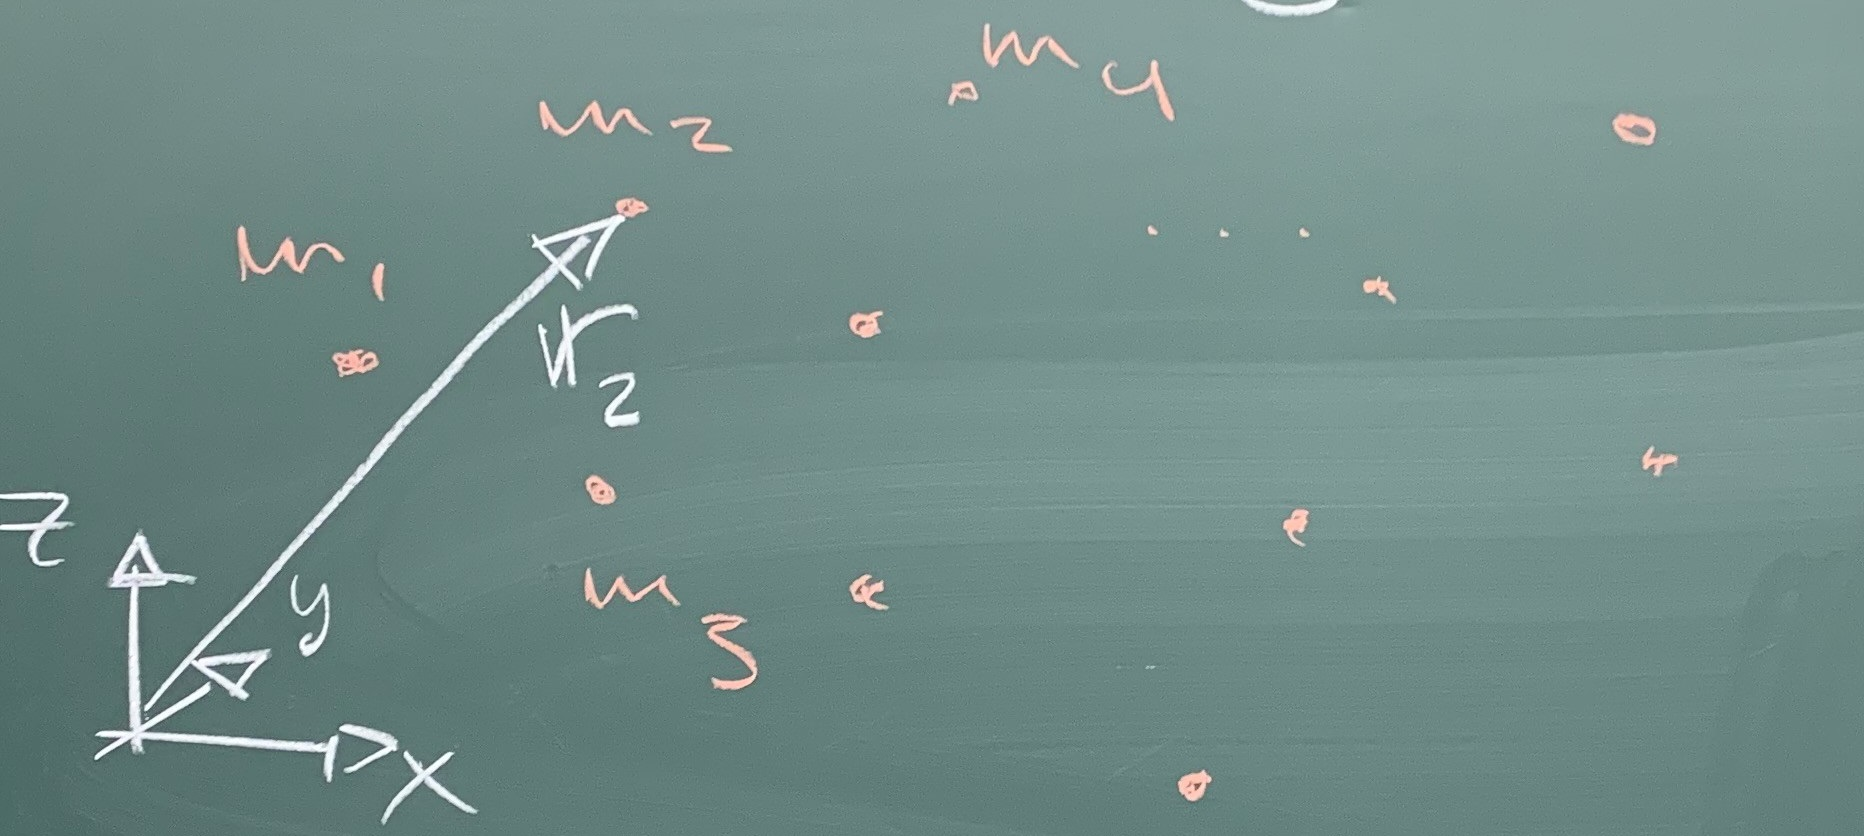
\includegraphics[scale=0.1]{lessons/lesson20/imgs/img01.jpg}\\
Systemets tyngdpunkt $\overline{r}$ definieras som:
\begin{equation*}
    \overline{r}=\frac{\sum_i r_i\cdot m_i}{\sum_i m_i}
\end{equation*}
Systemets moment betecknas $M_0$ och består av tre dimensionskomponenter:
\begin{equation*}
    M_0=(M_{x=0},M_{y=0},M_{z=0})
\end{equation*}
Vad blir motsvarande för en stel kropp vars densitet i en punkt $(x,y,z)$ beskrivs av $\varrho (x,y,z)$.
Stel kropp:\\
%infoga bild 2
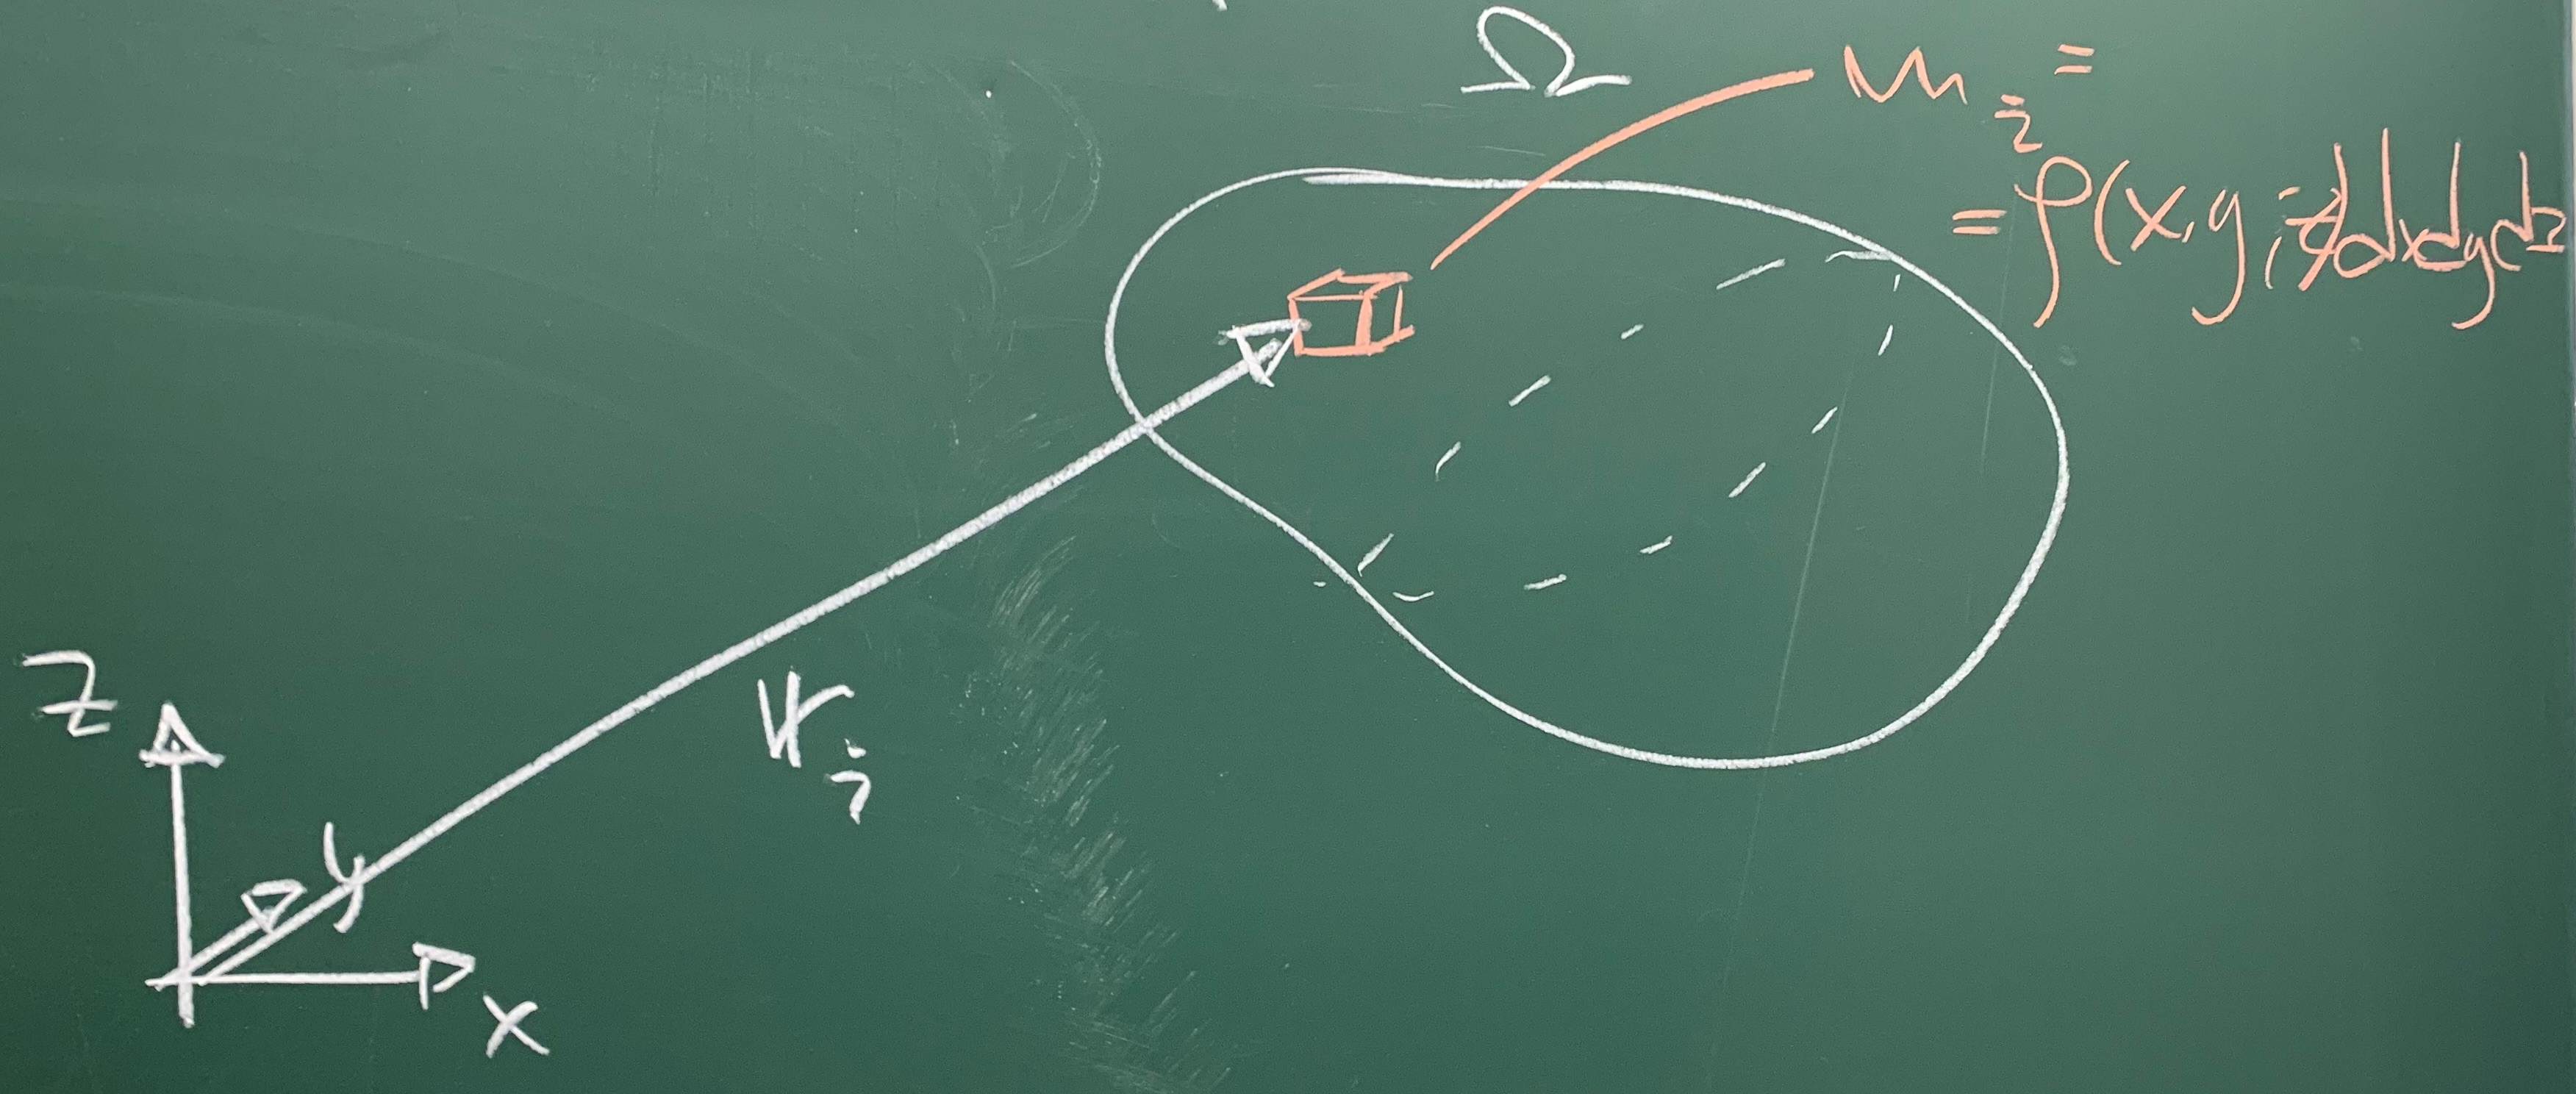
\includegraphics[]{lessons/lesson20/imgs/img02.jpg}\\
så tyngdpunkten för den stela kroppen blir:
\begin{equation*}
    \overline{r}=
    \sum_i \frac{m_i \overline{r}_i}{\sum_i m_i}\to
    \frac{\int_\Omega (x,y,z)\cdot\varrho(x,y,z)\, dx\, dy\, dz}{\int \varrho(x,y,z)\, dx\, dy\, dz}
\end{equation*}
Om man kan identifiera symmetrier ibland $\overline{r}$ beräknas med hjälp av "enkelintegraler".

\paragraph{Ex (7.4.7)} Beräkna tyngdpunkten för en kvadratisk platta med sidan $a$ cm om dess areadensitet är $\varrho(x)=k\cdot x$ g/cm$^2$ där $x$ är asvtåndet mellan en punkt $P$ på plattan och en av plattans sidor.
\subparagraph{Lösning}
Lägg plattan i ett koordinatsystem där "referenssidan" för plattans densitet är sammanfaller med y-axeln.\\
%infoga bild 3
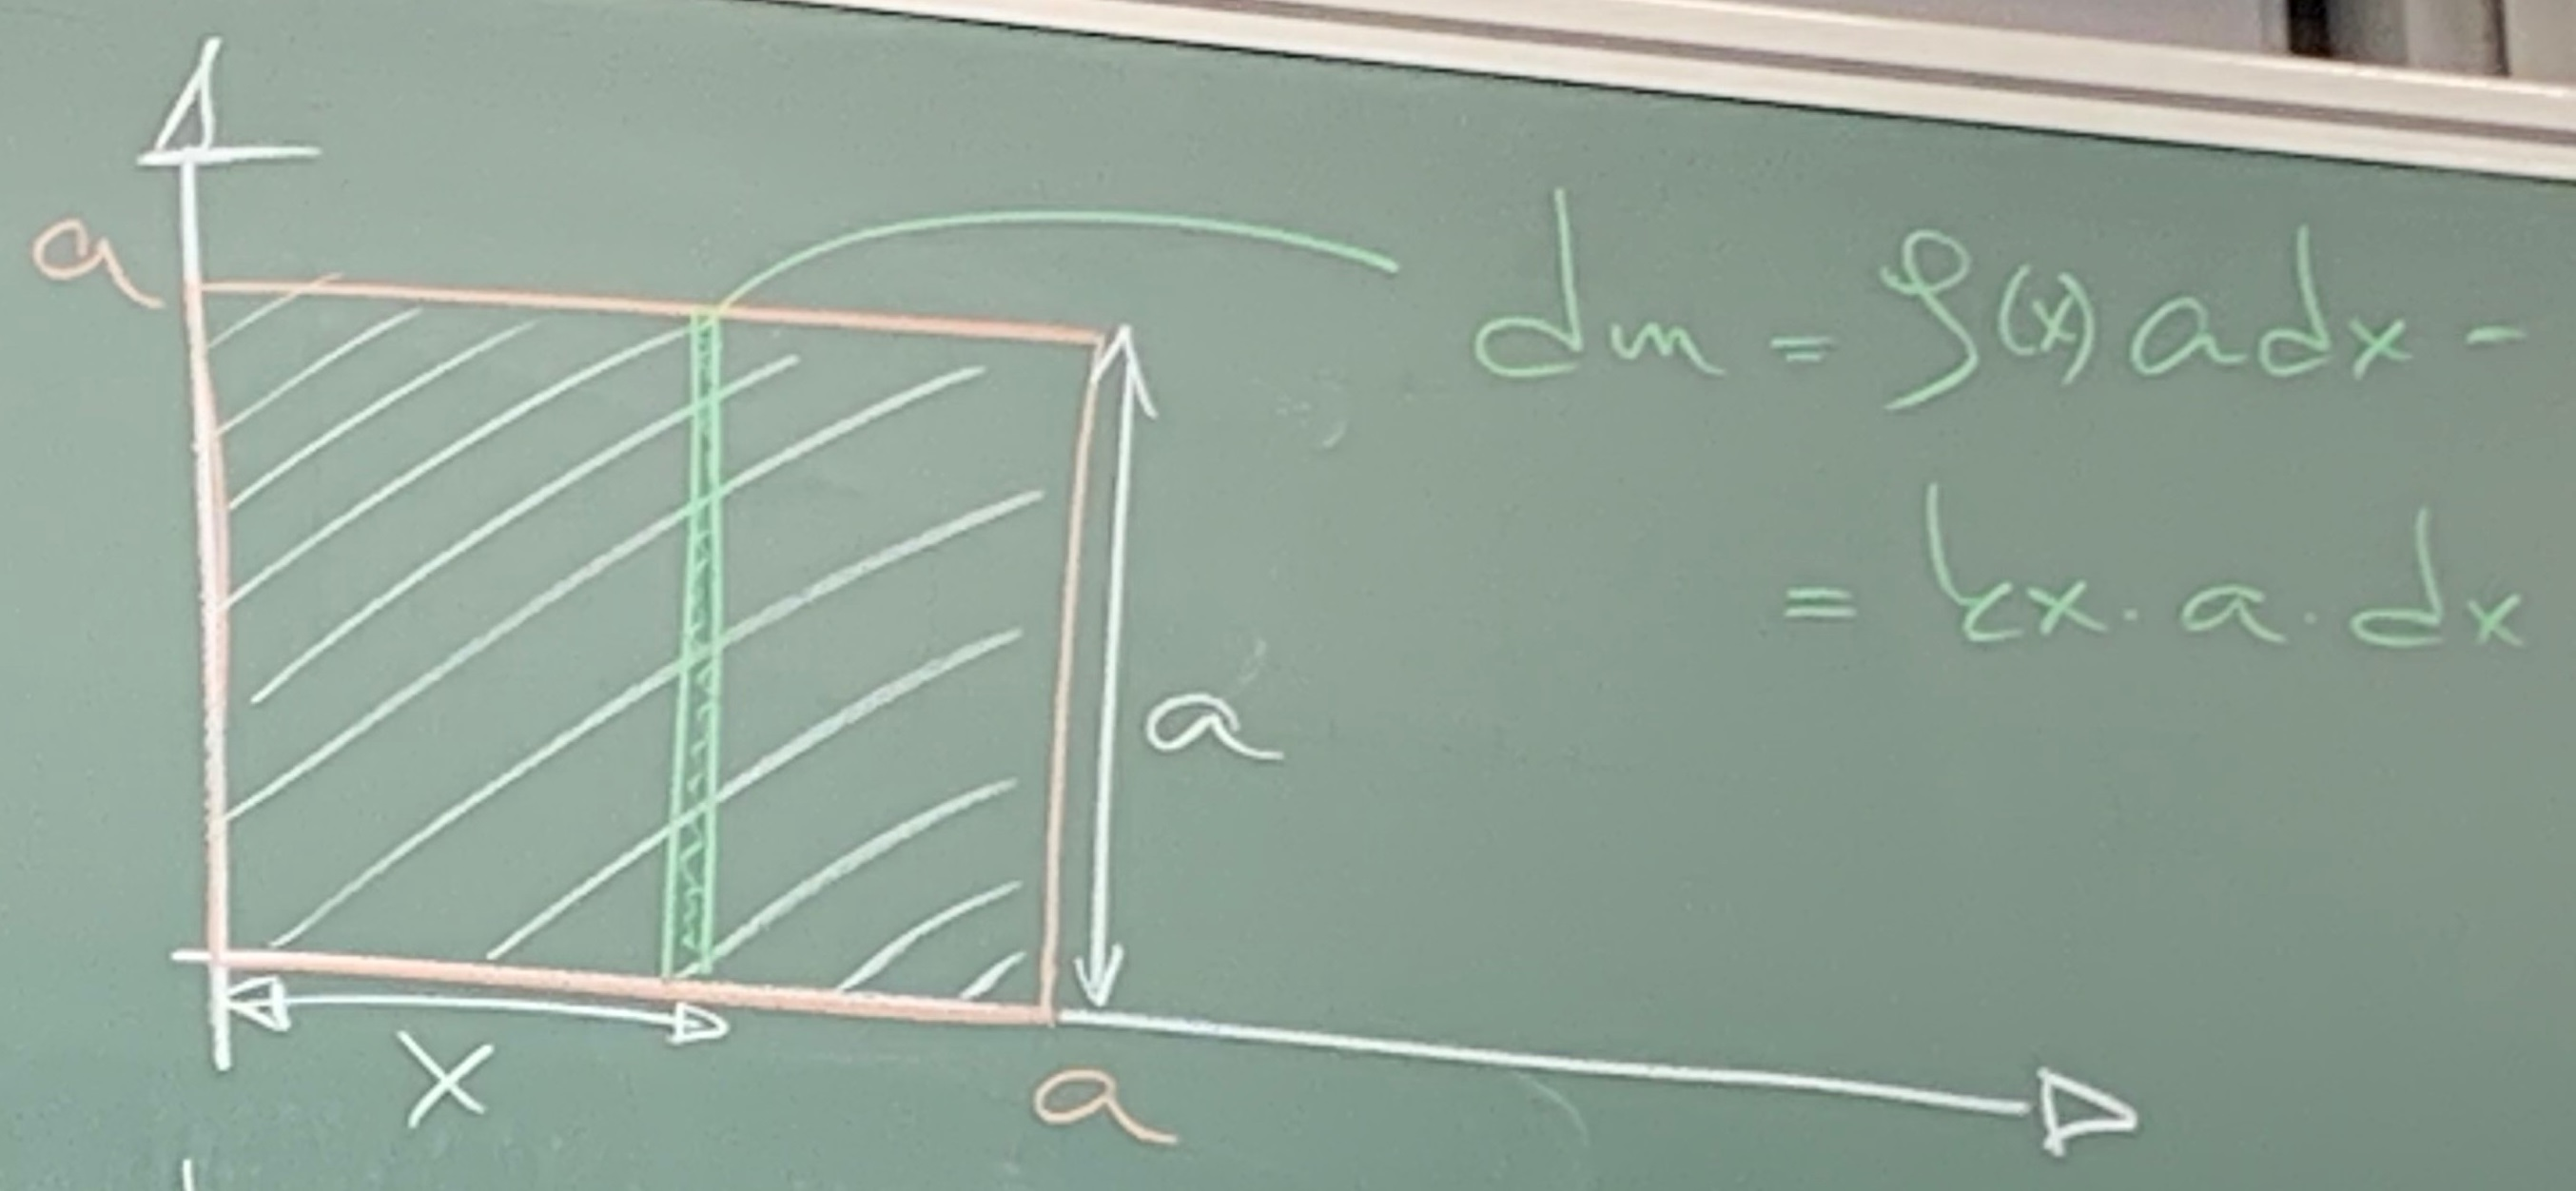
\includegraphics[scale=0.1]{lessons/lesson20/imgs/img03.jpg}\\
Uppenbart av symmetriskäl att tyngdpunkten i $y$-led ligger på höjden $\frac{a}{2}$.
Plattans totala massa $m$ blir:
\begin{equation*}
    m=\int dm=\int_0^a kx\cdot a\cdot\, dx=ka[\frac{x^2}{2}]_0^a=\frac{ka^3}{2}
\end{equation*}
Och momentet runt $x=0$ betecknas $M_{x=0}$, blir:
\begin{equation*}
    M_{x=0}=\int x\, dm=\int_0^a x\cdot kx\cdot a\cdot\, dx=ka[\frac{x^3}{3}]_0^a=\frac{ka^4}{4}
\end{equation*}
så tyngdpunkten i $x$-led hamnar i $\overline{x}=\frac{M_{x=0}}{m}=\frac{\frac{ka^3}{3}}{ka^3/2}=\frac{2a}{3}$
dvs. $\overline{r}=(\frac{2a}{3},\frac{a}{2}) \Box$

\paragraph*{Ex (7.4.14)} Beräkna tyngdpunkten för en boll med radie $R$ (m) om bollens densitet i en punkt $P$ är $\varrho(z)=z$ kg/m$^3$ där $z$ är asvtånd från $P$ till ett plan $2R$ m från bollems mittpunkt.
\subparagraph{Lösning}
% infoga bild 4
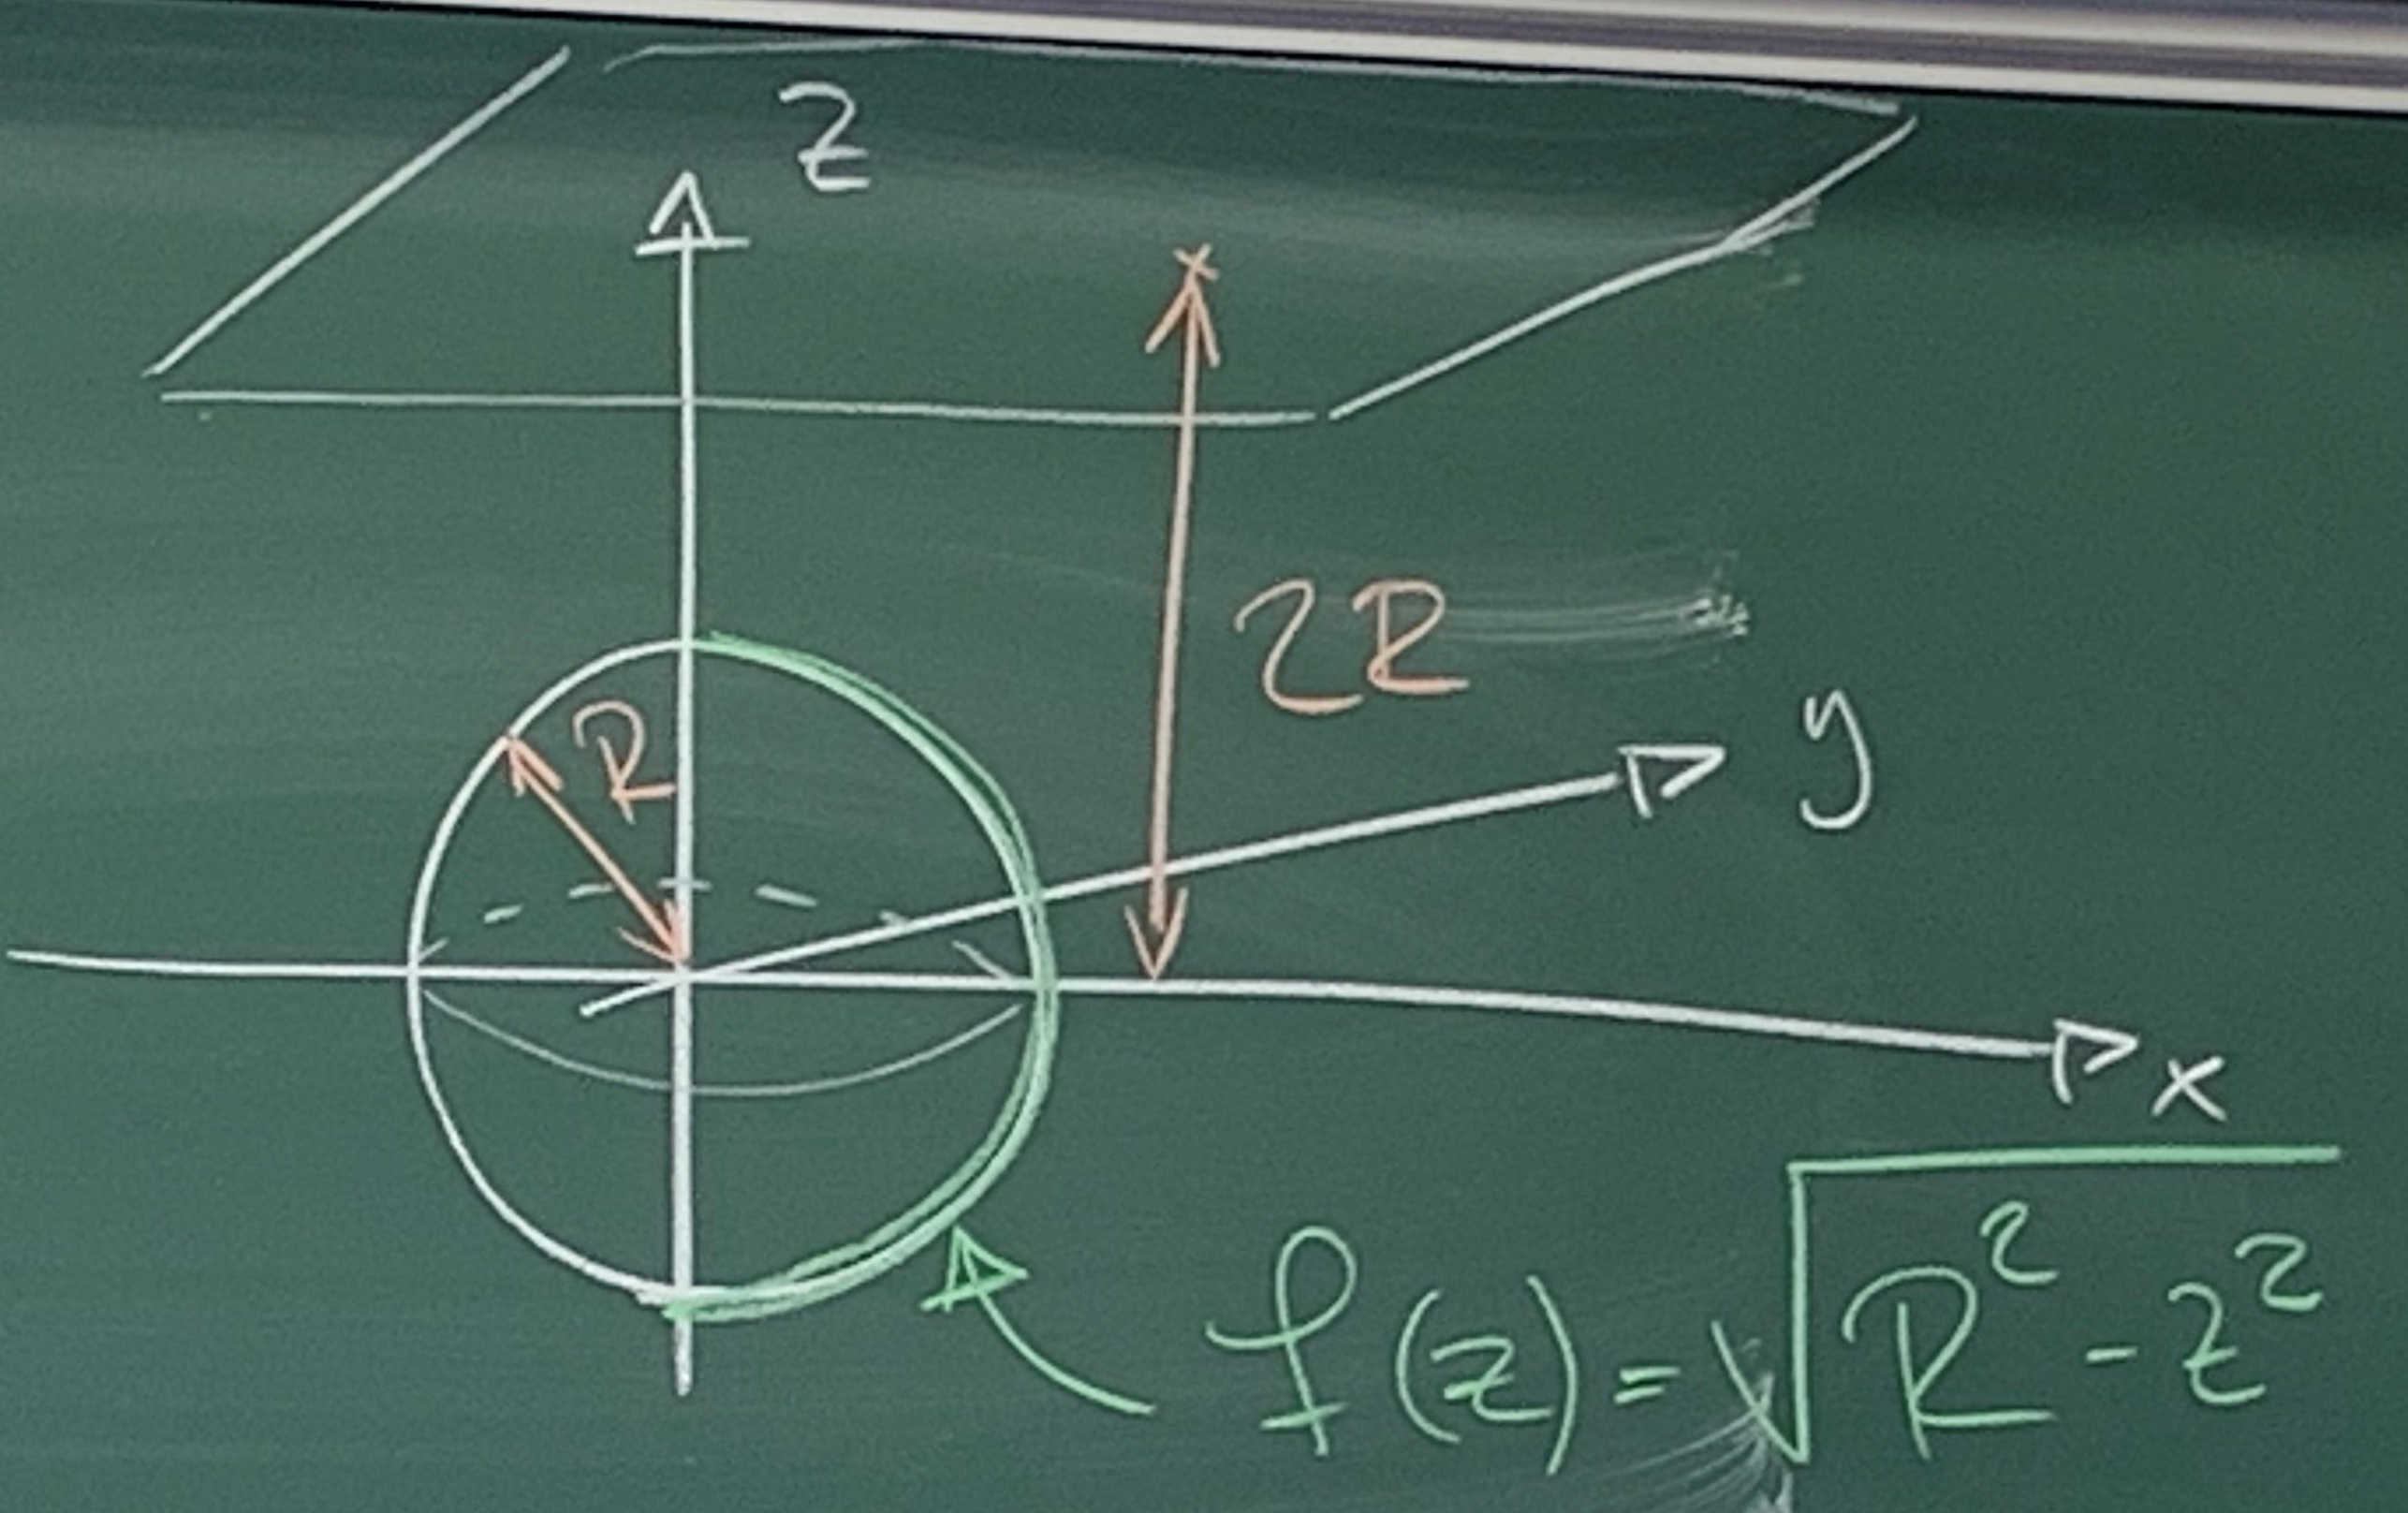
\includegraphics[scale=0.1]{lessons/lesson20/imgs/img04.jpg}\\
Med angivet koordinatsystem angivet enligt bild så är det givet att bollens tyngdpunkt i $x$- respektive $y$-led är $0$ på grund av symmetri och att densiteten endast varierar i $z$-led, dvs. $\overline{r}=(0,0,\overbrace{z})$.
Använd plattor parallella med  $xy$-planet för att beräkna $m$ och $M_{z=0}$.\\
% infoga bild 5
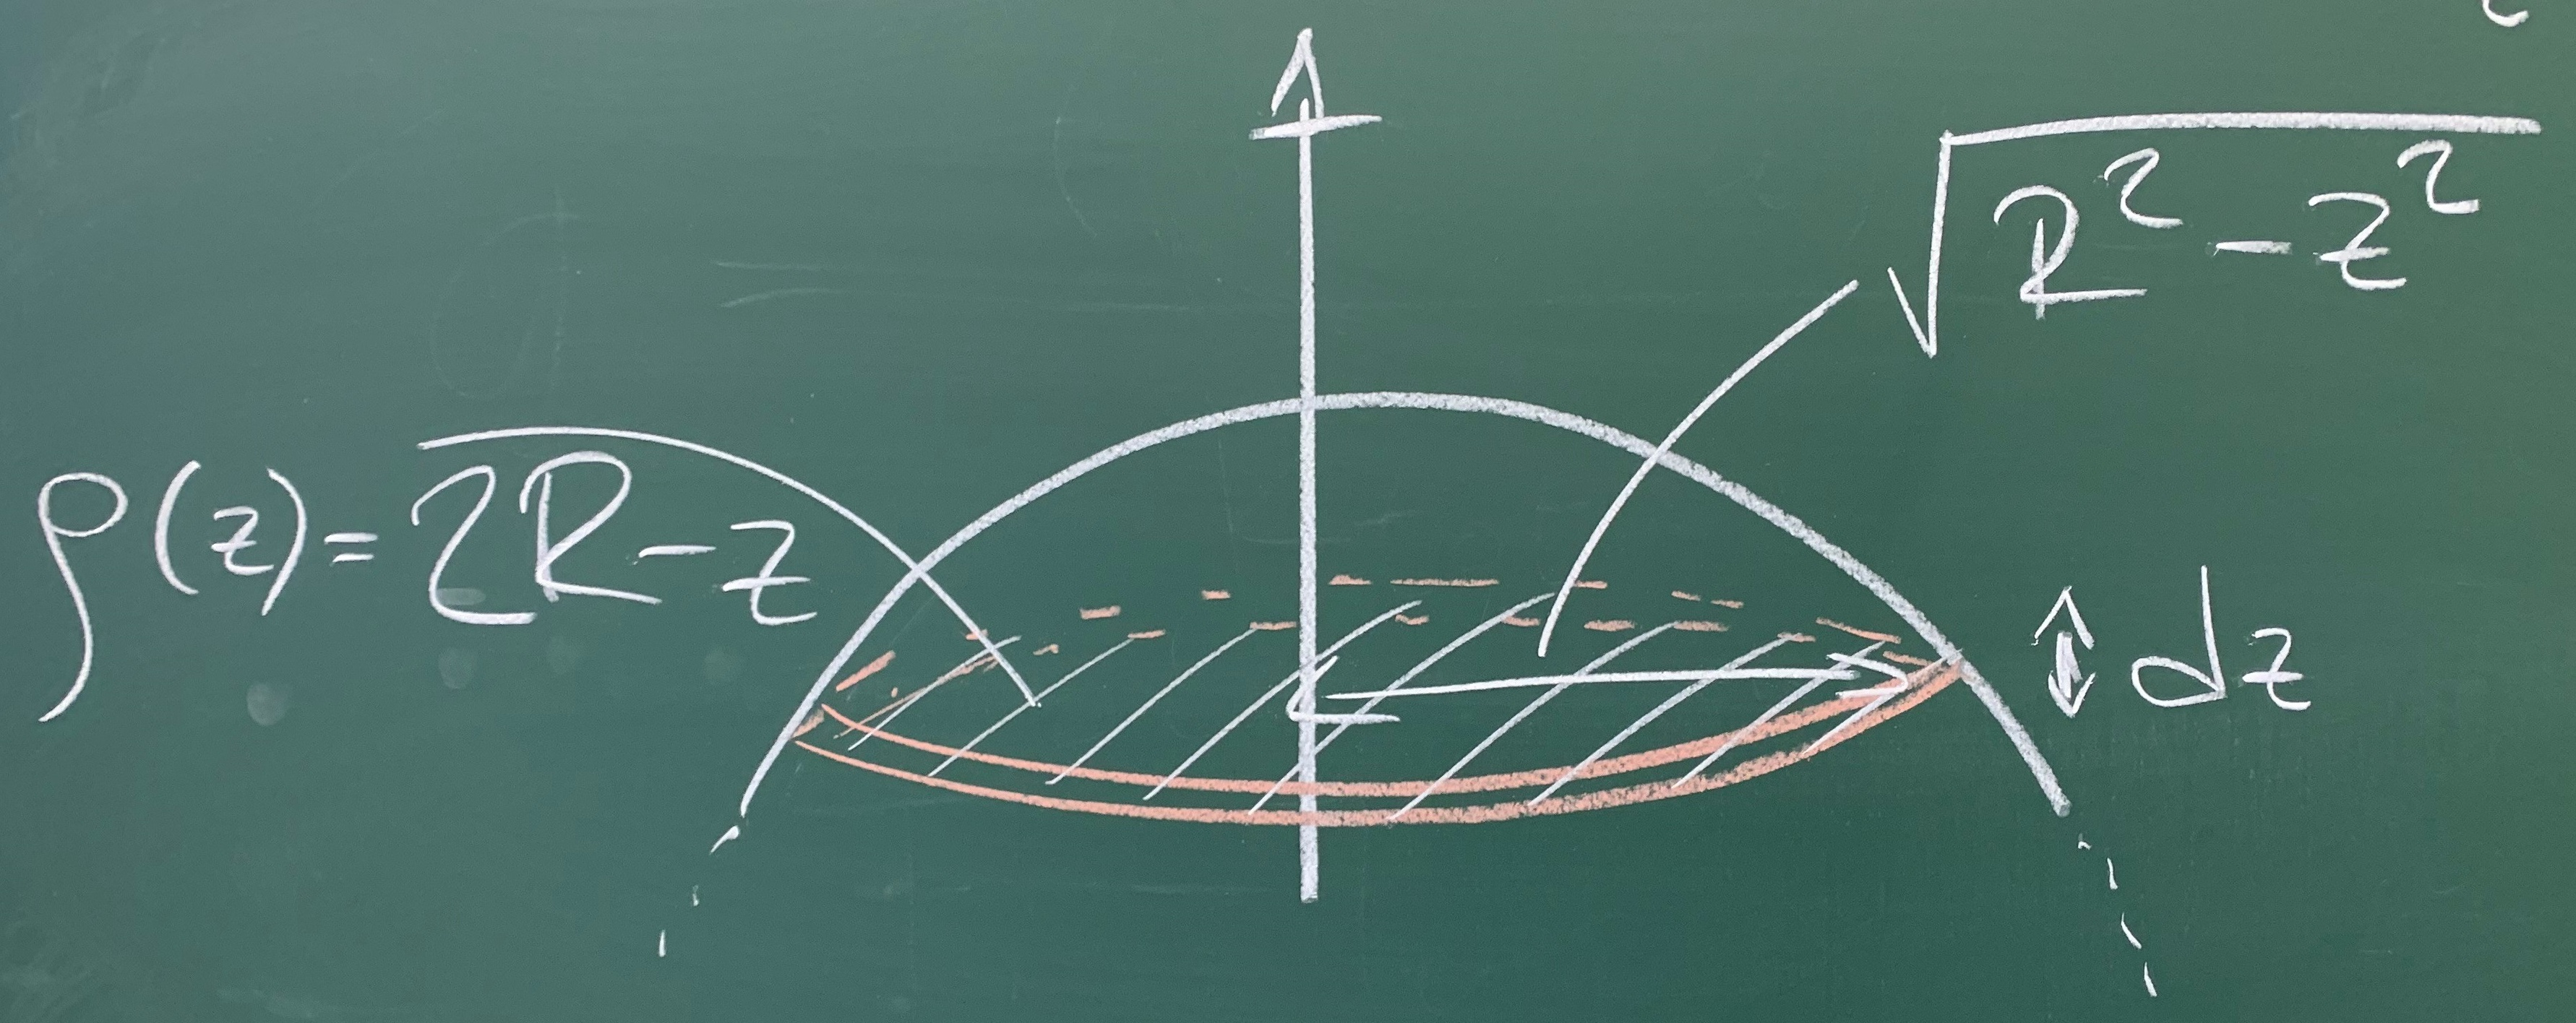
\includegraphics[scale=0.1]{lessons/lesson20/imgs/img05.jpg}
\begin{equation*}
    \Rightarrow dm=
    (2R-z)\cdot\pi(\sqrt{R^2-z^2})^2\, dz=
    \pi(2R-z)(R^2-z^2)\, dz
\end{equation*}
\begin{equation*}
    \Rightarrow m=
    \int dm=
    \int_{-R}^R\pi(2R-z)(R^2-z^2)\, dz=
    \pi\int_{-R}^R 2R^3-2Rz^2-zR^2+z^3\, dz=
\end{equation*}
\begin{equation*}
    \pi[2R^3z-\frac{2}{3}Rz^3]_{-R}^R=
    \frac{8}{3}\pi R^4
\end{equation*}
\begin{equation*}
    M_{z=0}=\int_{-R}^R z\, dm=
    \int_{-R}^R z\cdot\pi(2R-z)(R^2-z^2)\, dz=
    ...=
    \frac{4\pi}{15}R^5\Rightarrow
\end{equation*}
\begin{equation*}
    \overline{z}=\frac{4\pi\frac{R^5}{15}}{\frac{8\pi R^4}{3}}=
    ...=
    \frac{R}{10}\Box
\end{equation*}

\paragraph*{Ex (7.6.3)} En damm är $200$ m lång, $24$ m hög och är utformad som en $26$ m lång slip.
Om Vattenytan står vid dammens topp, hur stor kraft måste den då hålla emot från vattentrycket?
\subparagraph{Lösning}
%infoga bild 6
%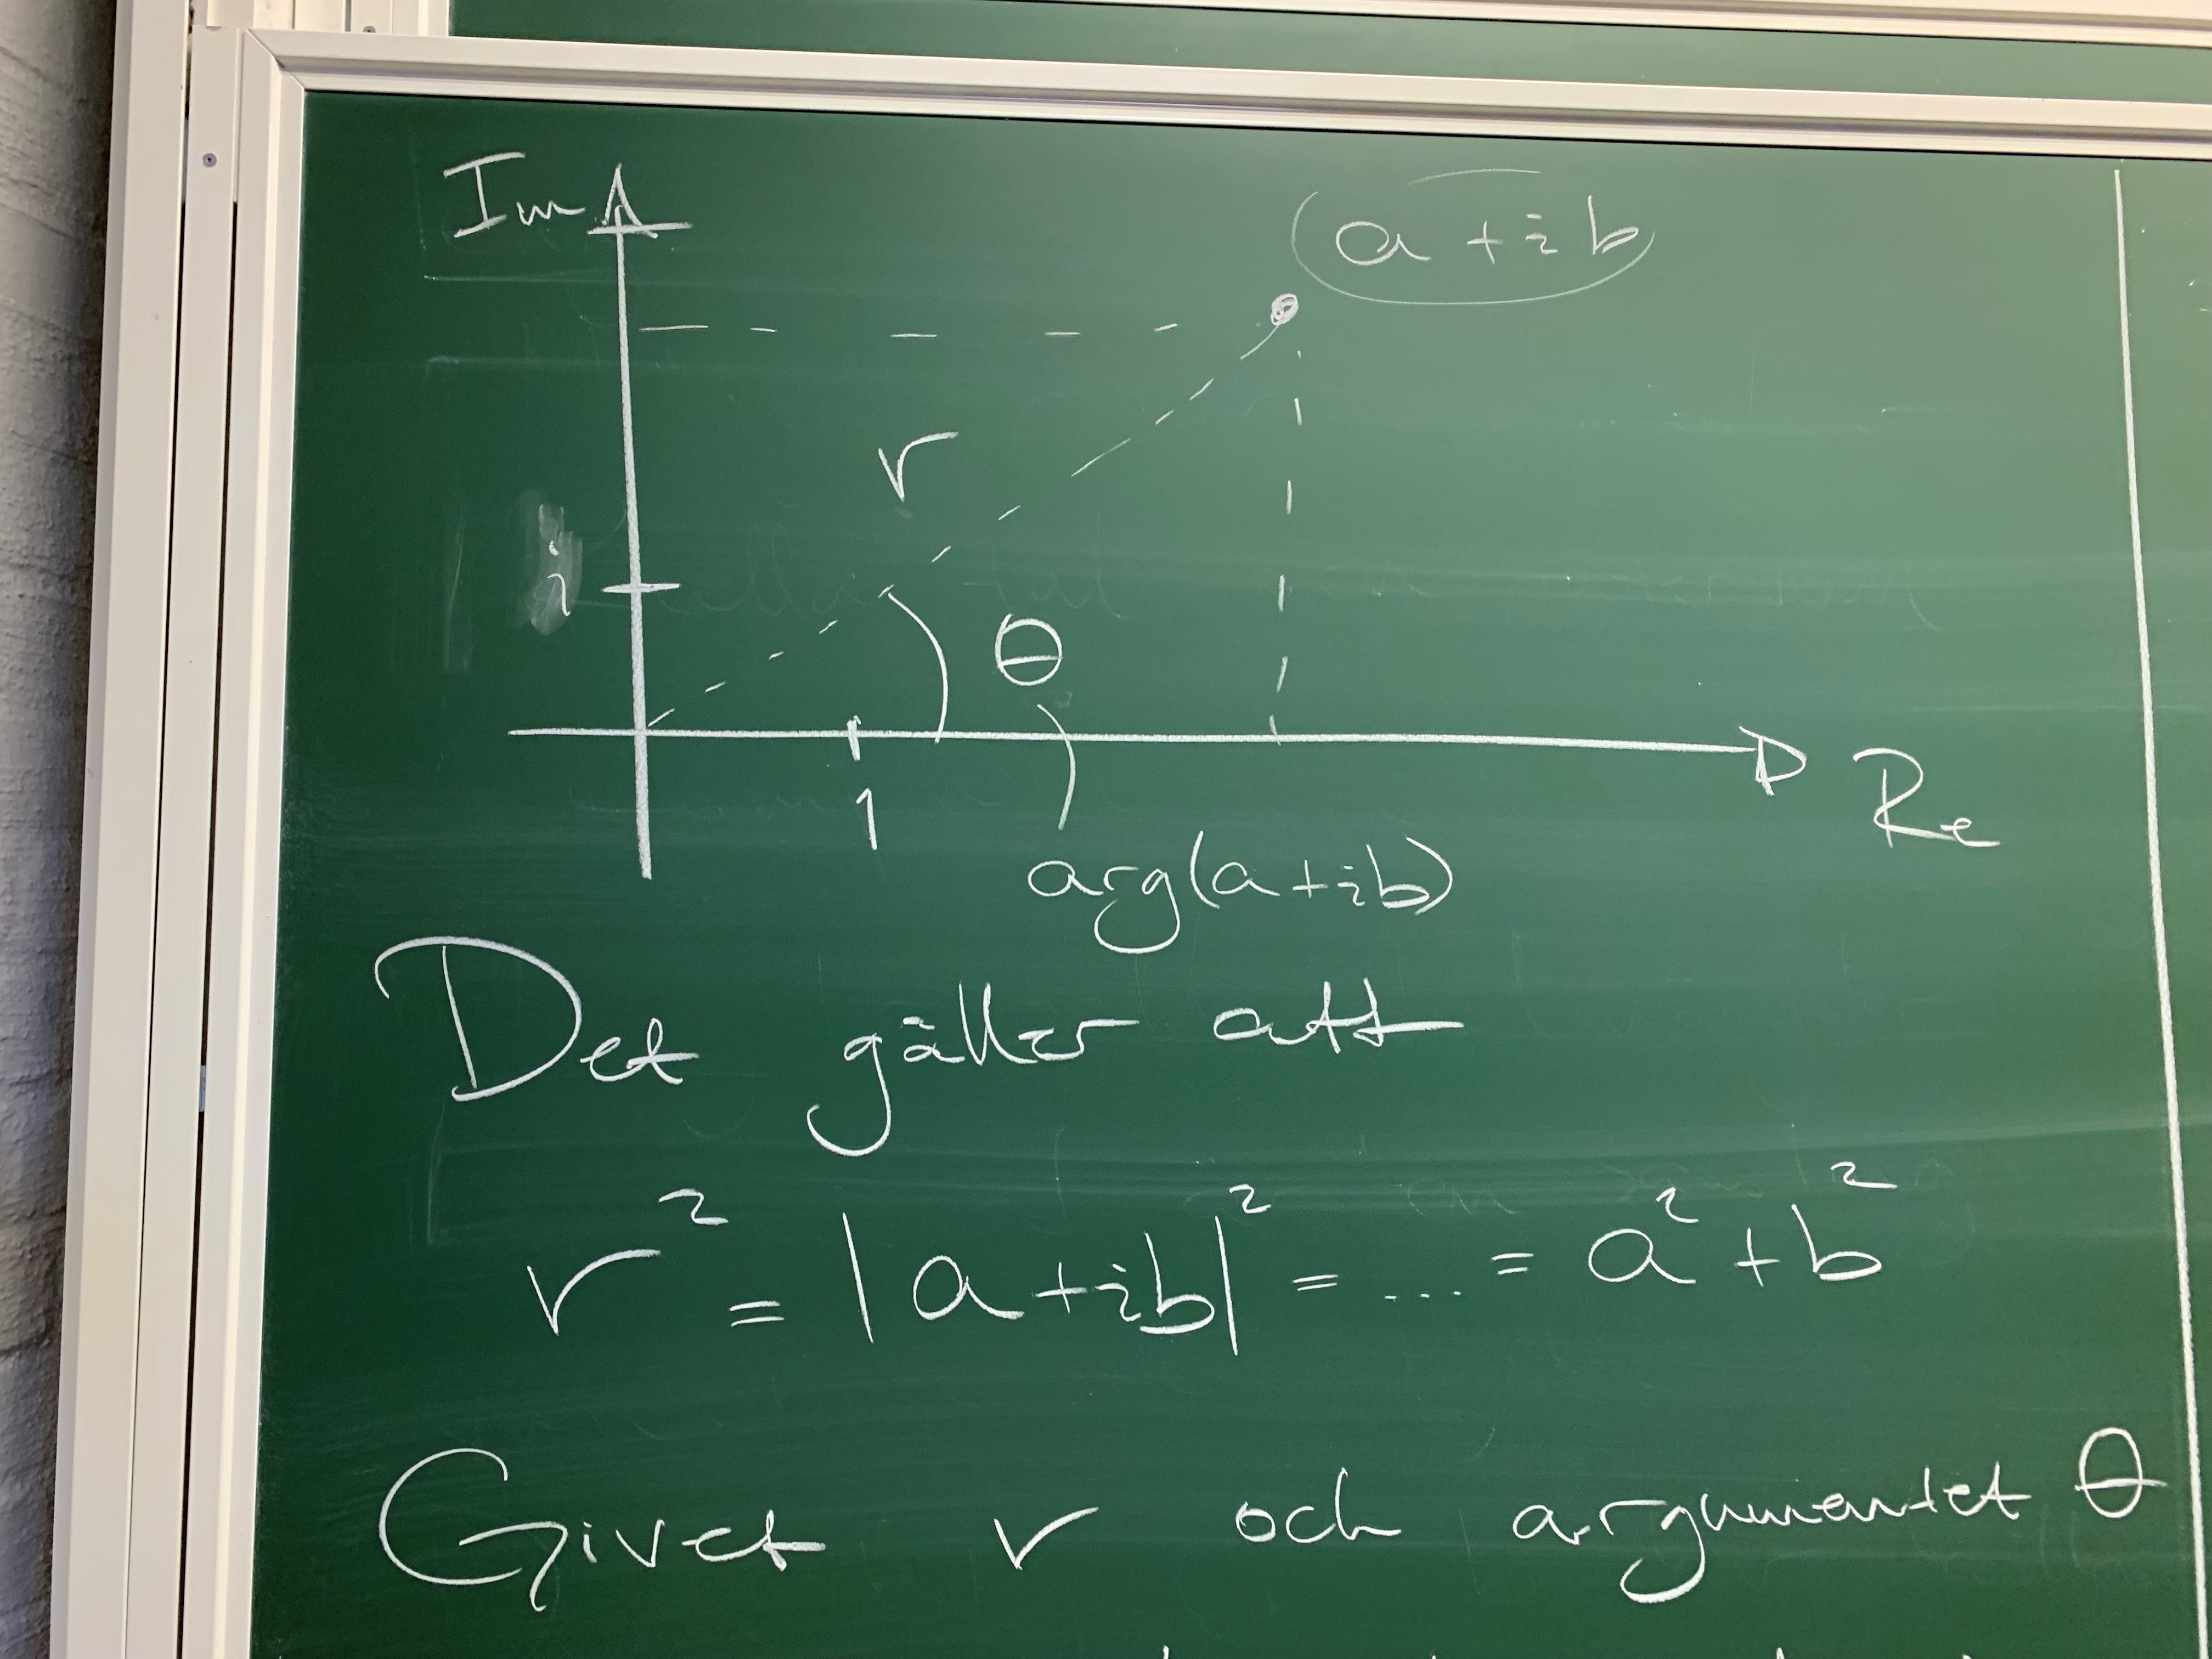
\includegraphics[scale=0.1]{lessons/lesson20/imgs/img06.jpg}\\
Det hydrostatiska trycket på djupet $h$ m ges av $p=\varrho\cdot g\cdot h$ där $\varrho$ är vattnets densitet och $g$ är tyngdaccelerationen.\\
Betrakta en tunn delyta på dammen som kan betraktas som utsatt för ett konstant tryck.
Om ytans area är $dA$ så utsätts denna för en kraft $dF=p\cdot dA=\varrho g h\, dA$.
Vad är $dA$?\\
% infoga bild 7
%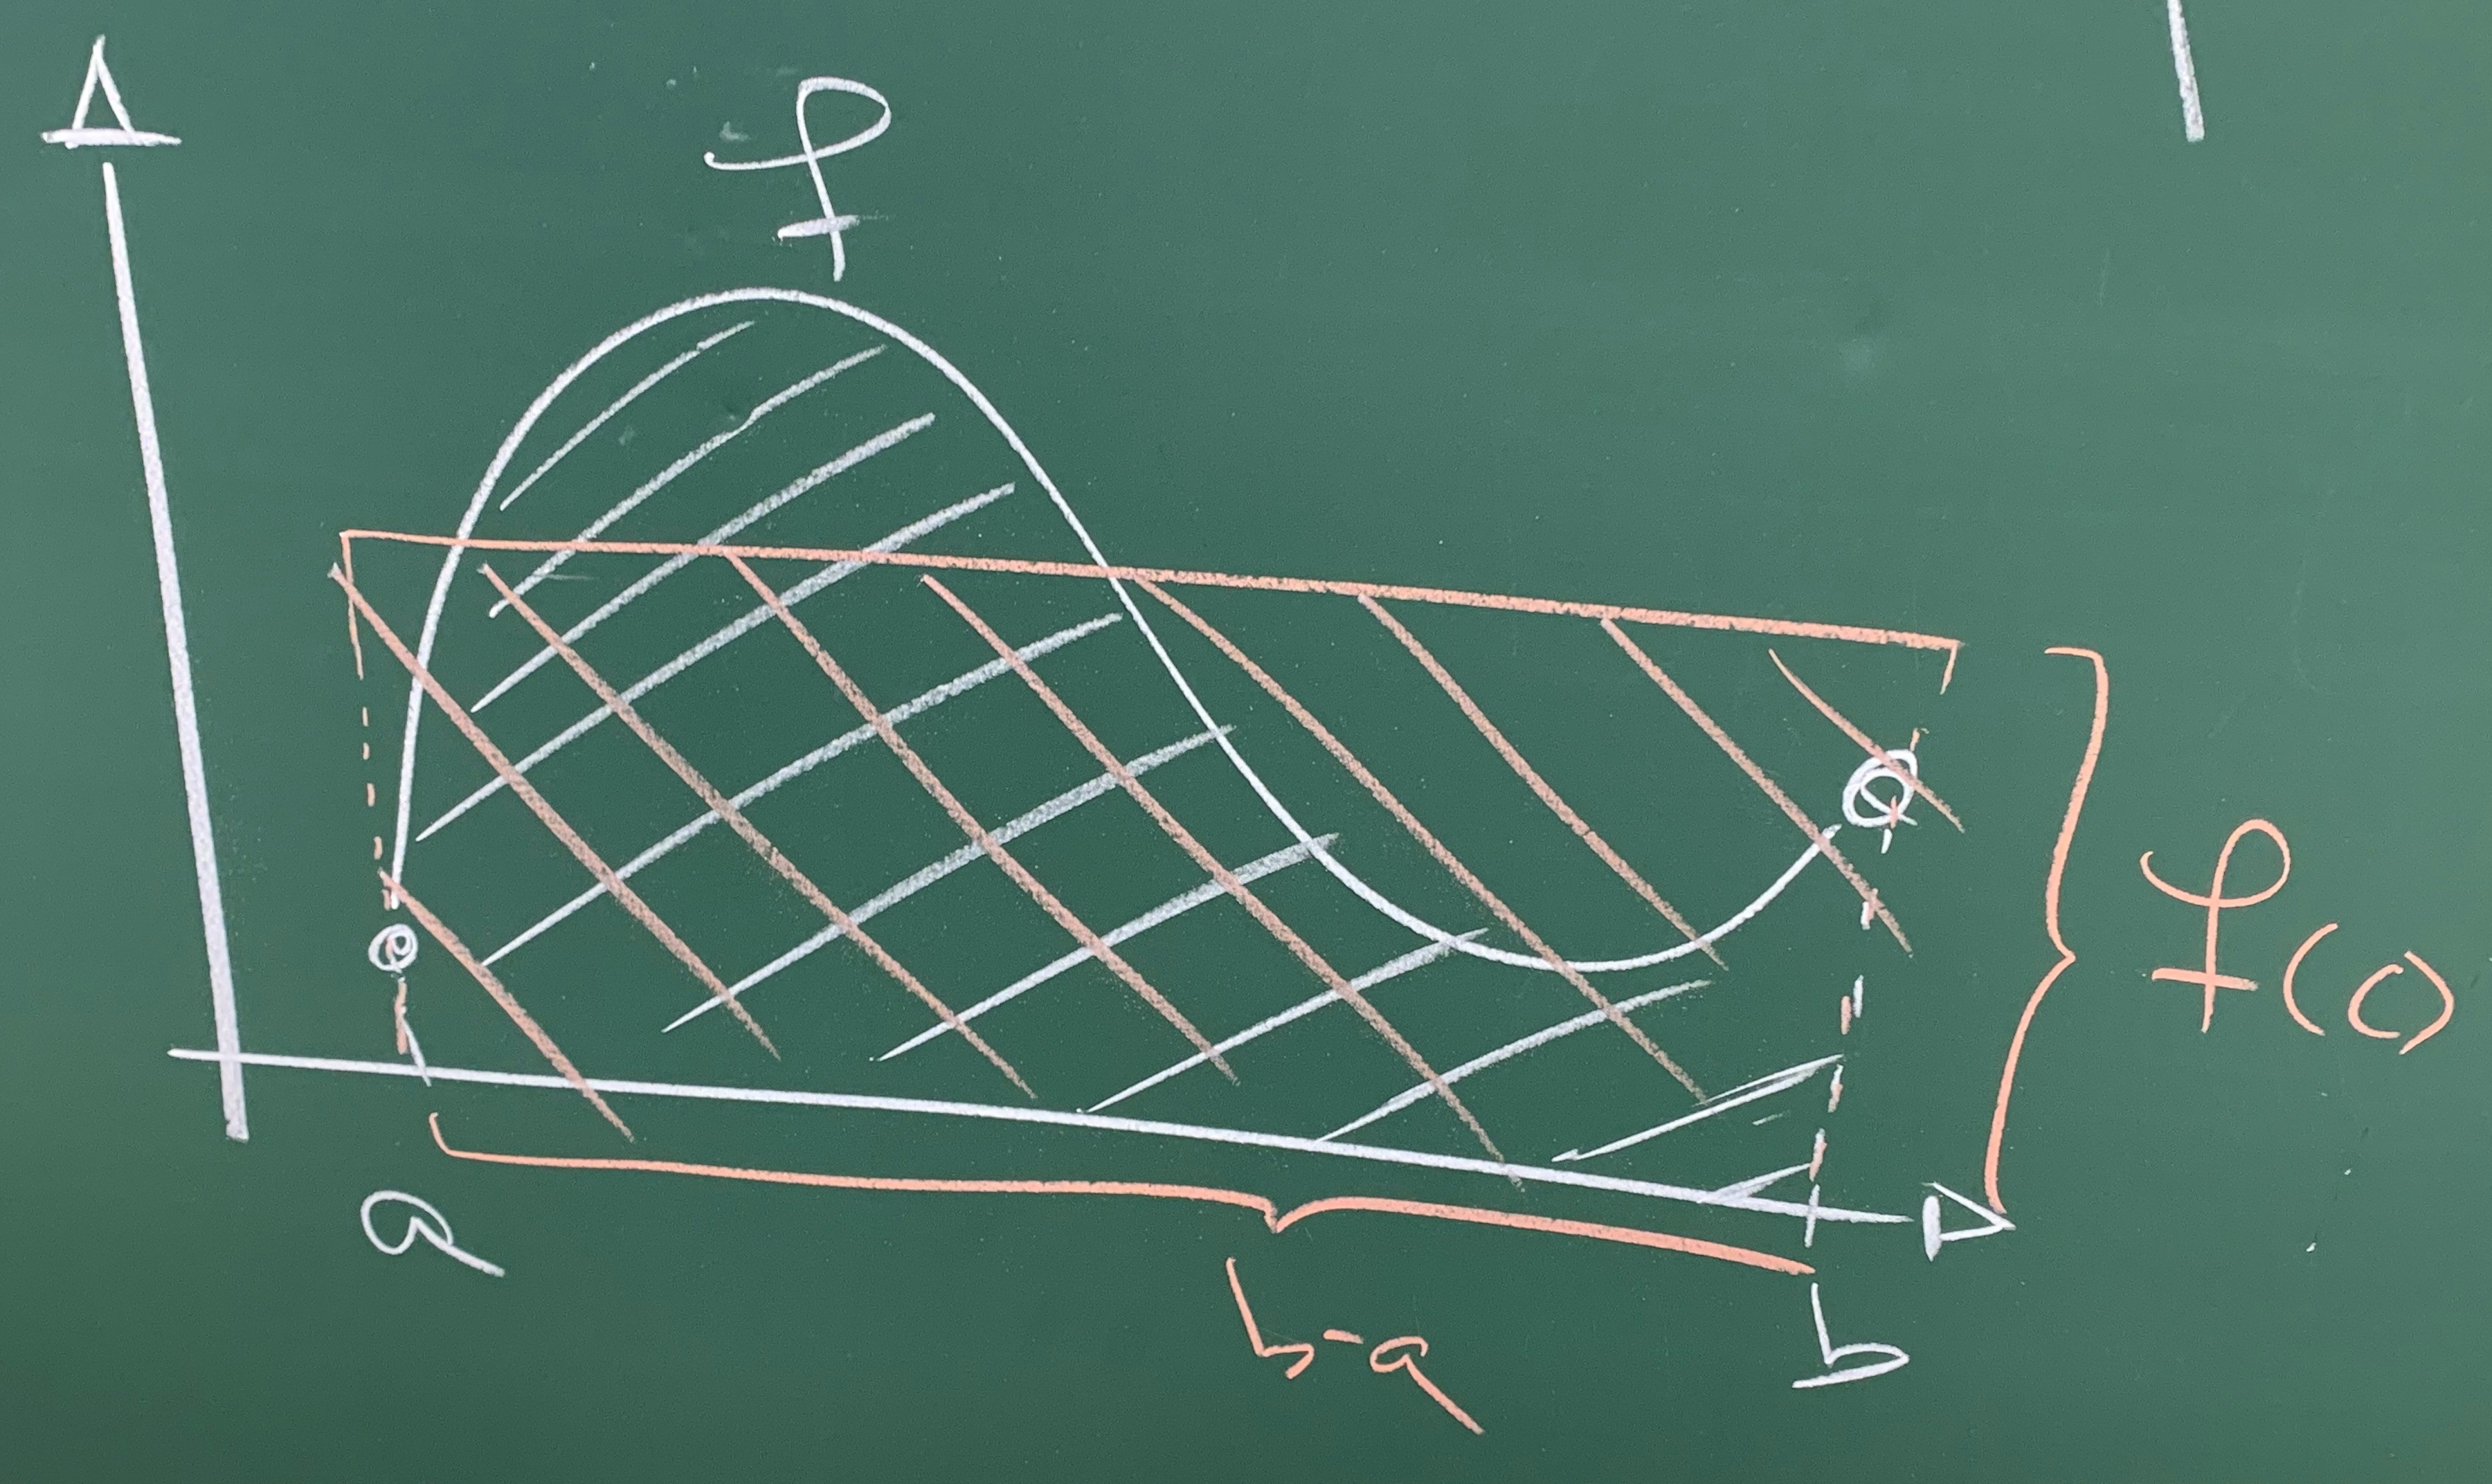
\includegraphics[scale=0.1]{lessons/lesson20/imgs/img07.jpg}
$dA=200\cdot ds=200\frac{dh}{\sin(\alpha)}$ där $\sin(\alpha)=\frac{24}{26}$ ($\Rightarrow\alpha\approx 67.4^\circ$) så
\begin{equation*}
    F_{\text{tot}}=
    \int dF=
    \int_0^24\varrho g h \cdot 200 \cdot\frac{dh}{\sin(\alpha)}=
    200\varrho g\frac{26}{24}\int_0^24h\, dh=
    200\varrho g\frac{26}{24}[\frac{h^2}{2}]_0^24=
    6.12\cdot10^8 \text{ N}
\end{equation*}

\paragraph{Ex (7.6.9)} Beräkkna det arbete som krävs för att pumpa allt vatten ur en (sfärisk) skål med radie $a$ m till en höjd $h$ m ovanför skålens top.
\subparagraph{Lösning}
%infoga bild 8
%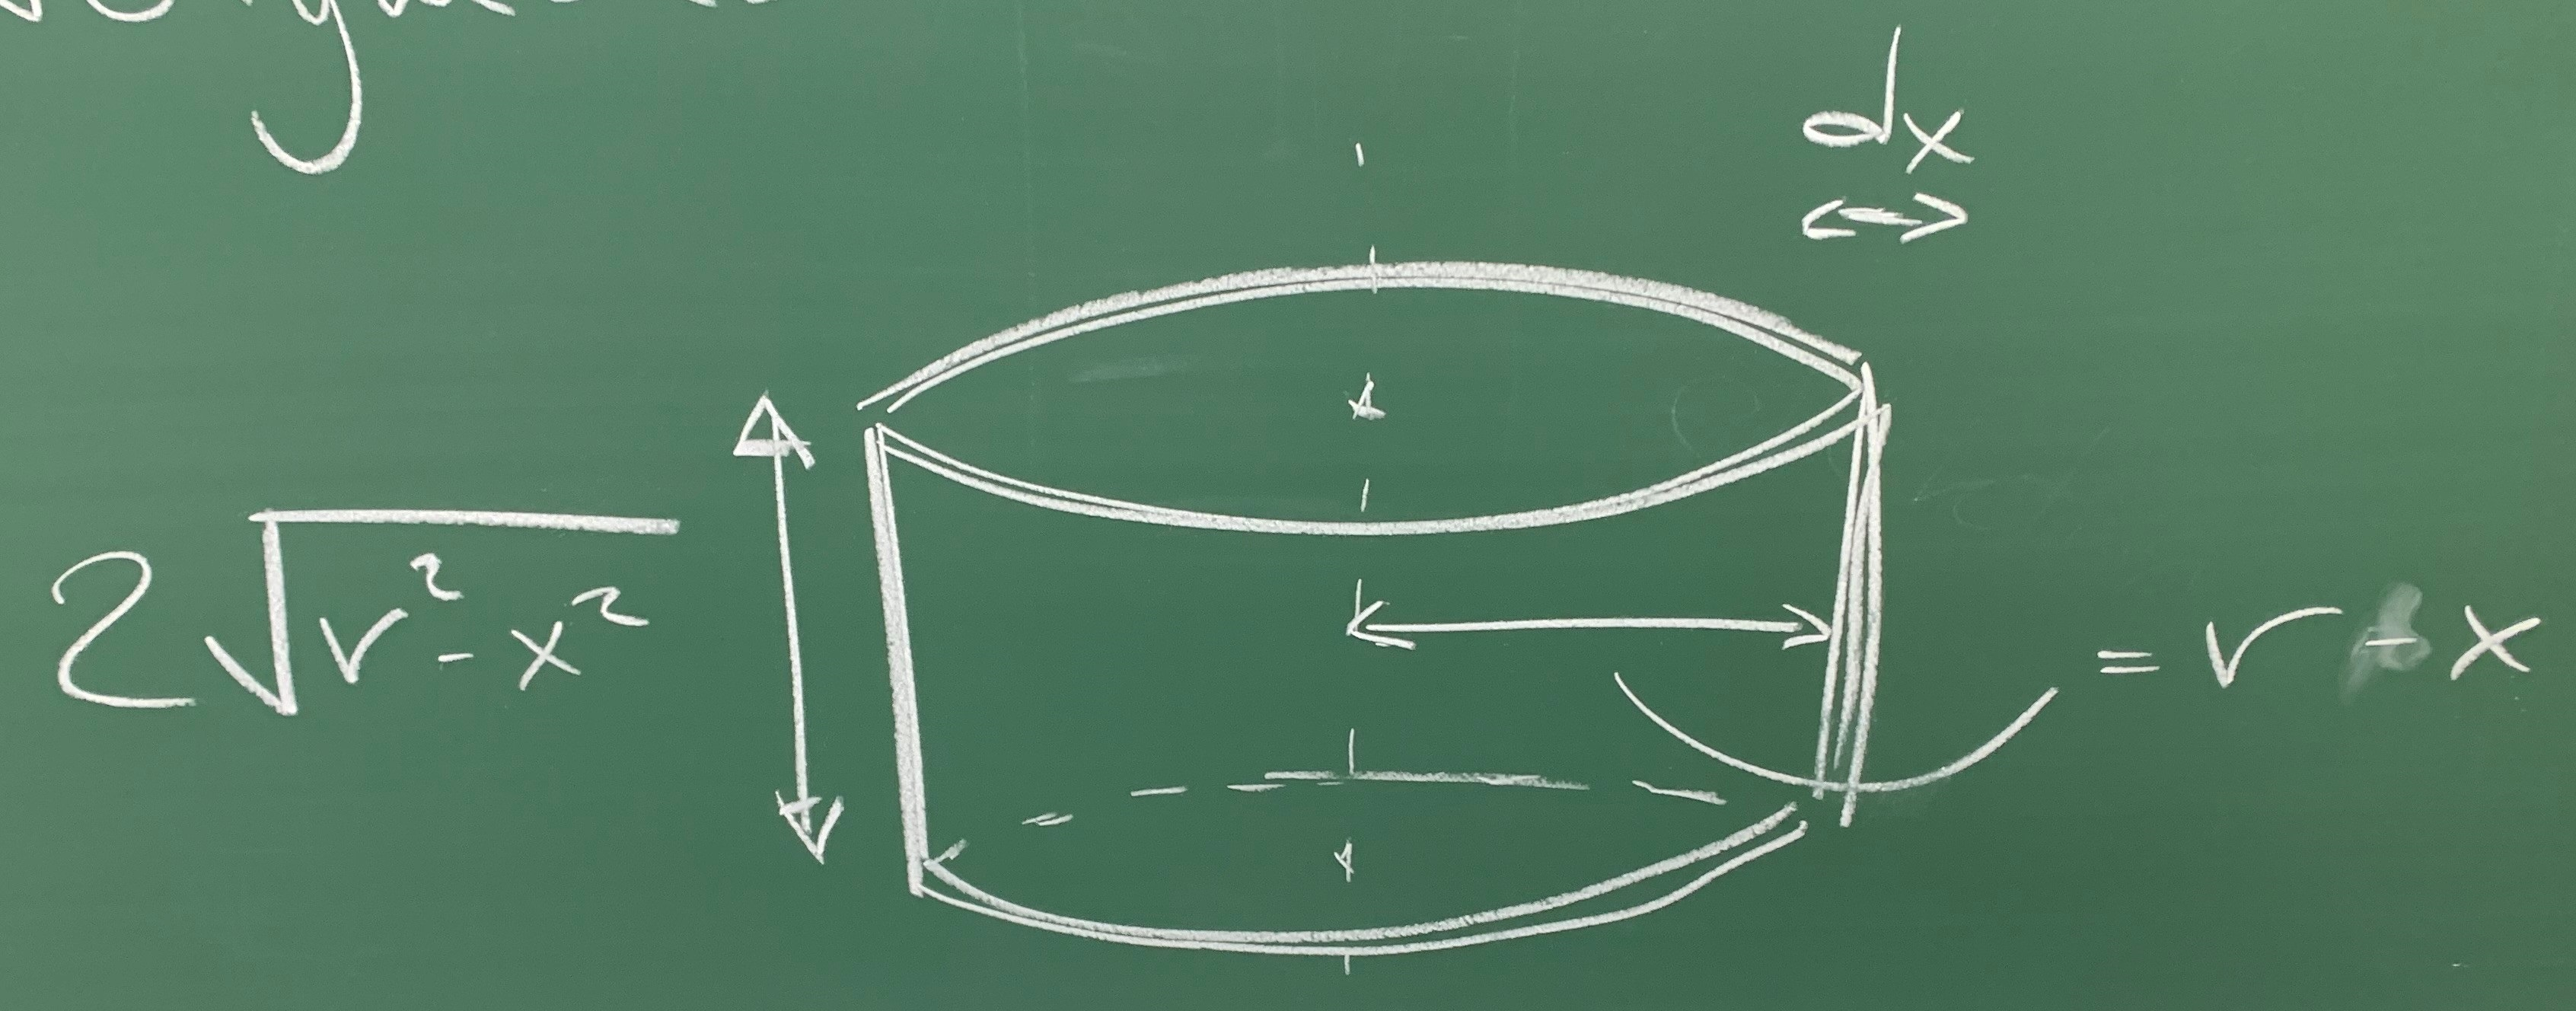
\includegraphics[]{lessons/lesson20/imgs/img08.jpg}
Beräkna det arbete som krävs för att lyfta en tunn cirkulär vattenskiva från skålen till höjden $h$ enligt bild.
För cirkelbågen gäller att
%infoga bild 9
\begin{equation*}
    \text{så }dm=
    \varrho dV=
    \varrho A(x)\, dx=
    \varrho\pi f^2(x)\, dx=
    \varrho\pi(a^2-x^2)\, dx
\end{equation*}
Arbete att lyfta en massa $m$ till höjden $h$  ges av $W=mgh$ och alltså
\begin{equation*}
    dW=
    \varrho g\pi(a^2-x^2)(x+h)\, dx=
    \varrho g\pi(a^2x+a^2h-x^3-xh^2)\, dx
\end{equation*}
För att lyfta skvian vid $x$ till höjden $h$ krävs det totala arbetet $W_{\text{tot}}$ enligt
\begin{equation*}
    W_{\text{tot}}=
    \int dW=
    \int_0^a\varrho g\pi(a^2x+a^2h-x^4-hx^2)\, dx=
\end{equation*}
\begin{equation*}
    \varrho g\pi[\frac{a^2}{2}x^2+a^2hx-\frac{x^4}{4}-\frac{h}{3}x^3]_0^a=
    \varrho g\pi(\frac{a^4}{2}+a^3h-\frac{a^4}{4}-\frac{a^3h}{3})=
    \varrho g\pi(\frac{a^4}{4}+\frac{2a^3h}{3})=
\end{equation*}
\begin{equation*}
    \frac{\varrho g\pi a^3}{4}(a+\frac{8h}{3})=
    2450\pi a^3(a+\frac{8h}{3})\text{ J}\Box
\end{equation*}